\documentclass{article}
\usepackage{listings}
\usepackage{xcolor}
\usepackage{graphicx} % Pacote para inclusão de imagens

% Margens esquerda, direita, cima e baixo
\usepackage[a4paper, left=2cm, right=2cm, bottom=3cm]{geometry}

% Para headers e footers
\usepackage{fancyhdr}
\pagestyle{fancy}


\fancyhf{} % clear all header and footer fields
% [C] - Centered, [L] - Left, [R] - Right, \\ é line break
\fancyfoot[L]{Probabilidade e Estatística 2024/25 - Projeto Ex01 \\ Alexandre Carapeto Delgado - ist1109441}		

% Remove header line
\renewcommand{\headrulewidth}{0pt}


\definecolor{backcolour}{rgb}{0.95,0.95,0.92}


\lstdefinestyle{mystyle}{
    backgroundcolor=\color{backcolour},   
	% Cor dos comentarios
    commentstyle=\color{gray},
	% Cor de keywords
    keywordstyle=\color{olive},
    numberstyle=\tiny\color{gray},
	% Cor de strings
    stringstyle=\color{purple},
    basicstyle=\ttfamily\footnotesize,
    breakatwhitespace=false,         
    breaklines=true,                 
    captionpos=b,                    
    keepspaces=true,                 
    numbers=left,                    
    numbersep=5pt,                  
    showspaces=false,                
    showstringspaces=false,
    showtabs=false,                  
    tabsize=2
}



\begin{document}
\vspace*{-3.5cm}
\huge{\sffamily \color{black}Resolução}
\lstset{style=mystyle}
\vspace{0.1cm}
\lstinputlisting[language=R]{/ex01.R}

\vspace{0.1cm}
\huge{\sffamily \color{black}Gráfico}
\nopagebreak
\vspace{0.1cm}
\begin{figure}[!h] % Inicia o ambiente figure com a opção [h] para indicar que a imagem deve ser posicionada aqui (opcional)
    \centering % Centraliza a imagem
    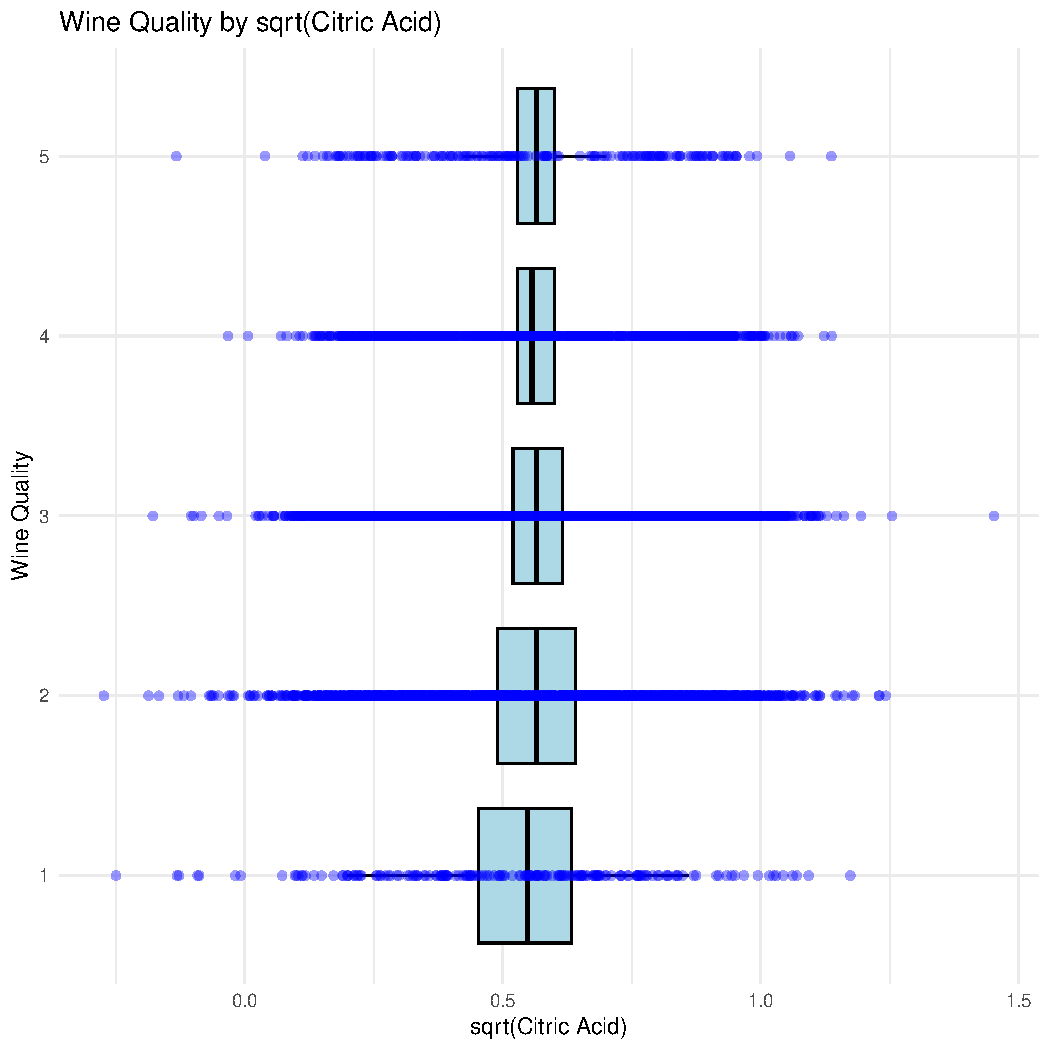
\includegraphics[width=0.8\textwidth]{Rplots.pdf} % Inclui a imagem "graph.jpg" com 50% da largura do texto
    \caption{Gráfico} % Adiciona uma legenda para a figura
    \label{fig:graph} % Adiciona uma etiqueta para referência cruzada
\end{figure}

\end{document}
